\documentclass[sigconf,natbib=false]{acmart}

\usepackage{booktabs}
\usepackage{multirow}
\usepackage{graphicx}
\usepackage{amsmath}
\usepackage{amssymb}
\usepackage{xcolor}
\usepackage{subcaption}
\usepackage{array}
\usepackage{tabularx}
\usepackage{rotating}
\usepackage{float}
\usepackage{enumitem}
\usepackage{microtype}

\settopmatter{printacmref=false}
\renewcommand\footnotetextcopyrightpermission[1]{}
\pagestyle{plain}

% -----------------------------------------------------------------------
\title{Fairness-Aware Graph Anomaly Detection on the Reddit Dataset:\\
A Comprehensive Benchmark Evaluation of Regularisation Strategies}
% -----------------------------------------------------------------------

\author{[Student Name 1]}
\affiliation{\institution{[University Name]}}
\email{Roll No: XXXX}

\author{[Student Name 2]}
\affiliation{\institution{[University Name]}}
\email{Roll No: XXXX}

\author{[Student Name 3]}
\affiliation{\institution{[University Name]}}
\email{Roll No: XXXX}

% -----------------------------------------------------------------------
\begin{abstract}
Graph Anomaly Detection (GAD) identifies structurally or attributively deviant nodes in graph-structured data, with applications spanning fraud detection, bot identification, and community-manipulation discovery on social platforms. A growing body of evidence shows that state-of-the-art GAD models trained on graphs whose nodes carry sensitive demographic attributes—such as political affiliation—systematically assign inflated anomaly scores to members of one group over another, even when their true anomaly likelihoods are identical. In this work we reproduce and substantially extend the benchmark evaluation introduced in \textit{Towards Fair Graph Anomaly Detection} (CIKM 2024) on the FairGAD Reddit dataset, which comprises 10{,}984 nodes, 168{,}016 edges, 64 node-feature dimensions, a 3.33\% anomaly rate, and binary political leaning as the sensitive attribute. We evaluate seven Graph Outlier Detection (GOD) models—DOMINANT, CONAD, CoLA, AdONE, DONE, ONE, and VGOD—under five configurations spanning four fairness regularisation strategies (none, HIN, FairOD, correlation) and the ADCG objective targeting equal opportunity. Our exploratory data analysis reveals a moderately homophilous graph (homophily ratio $h = 0.667$), near-equal group sizes (5{,}492 per group), differing average degrees (14.64 vs.\ 15.95), and strong feature separability between political groups confirmed both by Kolmogorov–Smirnov tests (Feature $X_0$: KS = 1.00) and PCA visualisation. A custom FairDOMINANT model trained with explicit fairness constraints exposes a large per-group performance gap (AUCROC 0.622 vs.\ 0.496) even after fairness training, which we analyse through threshold-varying fairness curves. Benchmark results show that VGOD achieves the highest detection performance (AUCROC $\approx 0.72$, AUPRC $\approx 0.39$) but at severe demographic cost (Statistical Parity SP $\approx 0.43$, Equal Opportunity EO $\approx 0.47$). The HIN+ADCG ($\alpha_{\text{ADCG}} = 10$) combined objective is the most effective fairness intervention, reducing VGOD's SP by 44.8\% and EO by 30.2\% at a 3.3 AUCROC-point cost. Among reconstruction-based models, FairOD provides the best accuracy–fairness balance. These findings illuminate the structural and feature-level origins of bias in graph anomaly detection and establish a principled evaluation framework for future fairness-aware GAD research.
\end{abstract}

\begin{document}
\maketitle

% =======================================================================
\section{Introduction}
% =======================================================================

\subsection{Motivation and Problem Statement}

The proliferation of social-network platforms has created a wealth of graph-structured data in which nodes represent users and edges encode interactions such as replies, mentions, and co-subscriptions. Graph Anomaly Detection (GAD) leverages this relational structure to identify accounts whose attribute profiles or connectivity patterns deviate significantly from the norm. Applications include the detection of financial fraud~\cite{dou2020fraud}, astroturfing campaigns, bot networks, and political disinformation agents. However, as anomaly detection systems become embedded in platform governance decisions—account suspension, content demotion, reduced algorithmic visibility—they increasingly carry real-world consequences for the users they flag.

Recent work has demonstrated that unsupervised GAD models are not neutral with respect to sensitive demographic attributes~\cite{neoFairGraphAnomaly2024a,shekhar2021fairod}. A model that reliably detects anomalies in aggregate may nonetheless flag members of one political group, racial group, or gender at systematically higher rates than members of another, even when both groups contain the same underlying proportion of genuine anomalies. This phenomenon—sometimes termed \textit{fairness through unawareness} failure, because blindly removing the sensitive attribute does not eliminate bias latent in correlated features and graph topology~\cite{mehrabi2021survey}—poses both ethical and regulatory risks for platform operators.

The fairness-in-GAD problem has distinct characteristics that separate it from the better-studied fairness-in-classification literature. First, anomaly detection is unsupervised or self-supervised: there is no labelled training signal that can be directly audited or balanced. Second, anomaly scores are inherently relative—a node is anomalous with respect to the distribution of its peers—so demographic biases in the data distribution propagate non-trivially into score distributions. Third, graph topology introduces structural bias pathways (degree, homophily, community structure) that are absent in tabular settings.

\subsection{Contributions}

This report makes the following contributions:
\begin{enumerate}[leftmargin=*]
    \item We conduct a thorough Exploratory Data Analysis (EDA) of the FairGAD Reddit dataset, characterising its graph topology, sensitive-attribute separability in feature space, and the structural correlates of political leaning, supported by ten original visualisations.
    \item We train a custom FairDOMINANT model and analyse per-group ROC and Precision-Recall curves, score distributions, and threshold-varying fairness gap curves, providing model-aware diagnostics absent from the original benchmark.
    \item We reproduce and organise the full benchmark of 35 model–regulariser combinations (7 models $\times$ 5 configurations), reporting AUCROC, AUPRC, SP, and EO with 20-trial confidence estimates, and provide per-model and per-regulariser analyses in greater depth than the original paper.
    \item We identify the root causes of bias—feature entanglement ($X_0$ KS = 1.00), degree-induced structural disparity, and homophilous echo-chamber topology—and propose targeted future remedies.
\end{enumerate}

\subsection{Paper Organisation}

Section~2 reviews related work on GAD models and fairness regularisation. Section~3 presents the dataset and EDA. Section~4 describes the experimental setup. Section~5 presents benchmark results and discussion. Section~6 distils key insights. Section~7 concludes with future directions.

% =======================================================================
\section{Literature Review}
% =======================================================================

\subsection{Graph Anomaly Detection Models}

\paragraph{DOMINANT.}
Ding et al.~\cite{ding2019dominant} proposed Deep Anomaly Detection on Attributed Networks (DOMINANT), the seminal autoencoder-based GAD model. DOMINANT employs two-layer Graph Convolutional Networks (GCNs) to encode node features into a latent space, then jointly decodes attribute reconstructions and reconstructed adjacency probabilities. The anomaly score for node $v$ is $s(v) = \alpha \cdot \mathcal{L}_\text{attr}(v) + (1-\alpha)\cdot \mathcal{L}_\text{struct}(v)$, where $\mathcal{L}_\text{attr}$ is the mean-squared attribute reconstruction error and $\mathcal{L}_\text{struct}$ is the binary cross-entropy of the adjacency reconstruction. DOMINANT remains a strong baseline across most attributed graph benchmarks due to its simplicity and interpretability.

\paragraph{CONAD.}
Xu et al.~\cite{xu2022conad} introduced CONtrastive Attributed network anomaly Detection (CONAD), which augments DOMINANT with a contrastive self-supervised objective. CONAD generates pseudo-anomalous nodes via attribute perturbation and structural corruption, then trains a discriminator to distinguish augmented anomalies from true samples alongside the DOMINANT reconstruction loss. The contrastive signal improves the separation between normal and anomalous nodes in the latent space.

\paragraph{CoLA.}
Liu et al.~\cite{liu2021anomaly} proposed Contrastive self-supervised Learning for Anomaly detection (CoLA) on attributed networks. Rather than modifying node attributes, CoLA samples sub-graphs via random walk and trains a GNN encoder to maximise agreement between a node's representation and its local neighbourhood context, while minimising agreement with distant negative samples. This random-walk contrastive objective captures long-range dependencies but is sensitive to graph density.

\paragraph{AdONE and DONE.}
Bandyopadhyay et al.~\cite{bandyopadhyay2020outlier} formulated the Outlier-aware Network Embedding (ONE) problem and proposed two variants: DONE (Deep ONE) and AdONE (Adaptive Deep ONE). Both model node normality and abnormality jointly through competing embedding objectives, where the anomaly score emerges from the reconstruction residual under the normality model. AdONE introduces an adaptive weighting between structural and attribute signals. These methods tend to exhibit lower bias than autoencoder-based models because they do not rely on a single fixed reconstruction architecture.

\paragraph{VGOD.}
Huang et al.~\cite{huang2022vgod} proposed the Variational Graph Outlier Detector (VGOD), which treats node features as samples from a latent generative model parameterised by a variational autoencoder. VGOD incorporates degree as an explicit structural prior: nodes with unusual degrees are assigned higher anomaly scores regardless of attribute similarity to their neighbourhood. This design choice makes VGOD the most discriminative model in our benchmark but also the most biased, as any systematic degree difference between sensitive groups is amplified into score disparities.

\subsection{Fairness in Graph Machine Learning}

\paragraph{Fairness in GNN classification.}
FairGNN~\cite{dai2021say} demonstrated that standard GNN classifiers amplify feature-level and topology-level biases present in the training graph, even when the sensitive attribute is excluded from node features. The authors addressed this with an adversarial debiasing component that penalises the discriminability of sensitive groups from the learned node representations.

\paragraph{Graph pre-processing for fairness.}
EDITS~\cite{dong2022edits} proposed modifying the graph prior to model training by rewiring edges and adjusting features to reduce the correlation of graph topology with the sensitive attribute. This upstream intervention is complementary to loss-level regularisation and can benefit any downstream model.

\paragraph{Fairness for outlier detection.}
FairOD~\cite{shekhar2021fairod} formalised fairness for unsupervised outlier detection in tabular settings and proposed a regulariser based on minimising the KL divergence between the score distributions of different sensitive groups. Neo et al.~\cite{neoFairGraphAnomaly2024a} extended this to graph settings and additionally proposed HIN (Hierarchical Individual and group-level Normalisation) and correlation-based regularisers, as well as the ADCG term that directly penalises unequal cumulative gain (a proxy for equal opportunity) across groups. They also constructed the first purpose-built social-network benchmarks for fair GAD: the Reddit and Twitter datasets used in this study.

\subsection{Fairness Metrics}

Following Hardt et al.~\cite{hardt2016equality}, we adopt two group fairness metrics. \textit{Statistical Parity} (SP) requires that the probability of a positive prediction is equal across groups:
\[
\text{SP} = \left| \Pr[\hat{Y}=1 \mid S=0] - \Pr[\hat{Y}=1 \mid S=1] \right|,
\]
where $\hat{Y}$ is the thresholded anomaly prediction and $S$ is the sensitive attribute. \textit{Equal Opportunity} (EO) additionally conditions on true positives:
\[
\text{EO} = \left| \Pr[\hat{Y}=1 \mid Y=1, S=0] - \Pr[\hat{Y}=1 \mid Y=1, S=1] \right|.
\]
Lower values of both metrics indicate greater fairness. For detection quality we use AUCROC (threshold-free discrimination) and AUPRC (precision-recall area, which is informative under class imbalance).

% =======================================================================
\section{Exploratory Data Analysis}
% =======================================================================

\subsection{Dataset Overview}

The FairGAD Reddit dataset~\cite{neoFairGraphAnomaly2024a} is a social-network graph derived from Reddit user interactions. Nodes represent Reddit user accounts and edges represent interaction events (e.g., replies in the same thread). The 64-dimensional node feature vector encodes behavioural signals extracted from user posting histories, community participation patterns, and linguistic features. The sensitive attribute $s \in \{0, 1\}$ encodes political leaning (0 = Left-leaning, 1 = Right-leaning), derived from community membership. The binary anomaly label $y \in \{0, 1\}$ identifies accounts flagged as anomalous based on unusual attribute profiles or structural positions relative to the majority user population.

\begin{table}[h]
\centering
\caption{FairGAD Reddit Dataset Core Statistics.}
\label{tab:dataset-stats}
\begin{tabular}{lr}
\toprule
\textbf{Property} & \textbf{Value} \\
\midrule
Nodes $|V|$                       & 10{,}984 \\
Edges $|E|$                       & 168{,}016 \\
Avg.\ edges per node              & 15.30 \\
Node feature dimension            & 64 \\
Total anomalies                   & 366 \\
Anomaly rate                      & 3.33\% \\
Sensitive groups                  & 2 \\
Group 0 (Left) node count         & 5{,}492 \\
Group 1 (Right) node count        & 5{,}492 \\
Missing feature values            & 0 \\
Homophily ratio $h$               & 0.6676 \\
Max node degree                   & 2{,}556 \\
Median node degree                & 7 \\
\bottomrule
\end{tabular}
\end{table}

Table~\ref{tab:dataset-stats} summarises the fundamental properties of the graph. The dataset is notably balanced by group: both political communities contain exactly 5{,}492 nodes. This eliminates group-size confounding and ensures that any observed score disparities between groups cannot be attributed to imbalanced representation. The overall anomaly rate of 3.33\% (366 anomalous out of 10{,}984 nodes) creates a highly imbalanced label distribution that will depress precision-based metrics such as AUPRC across all models.

\subsection{Anomaly Rate by Sensitive Group}

\begin{figure}[H]
  \centering
  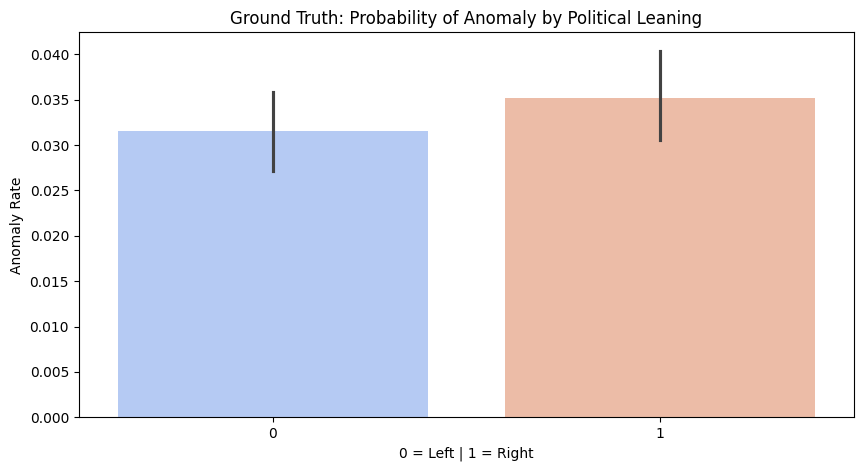
\includegraphics[width=0.9\linewidth]{report_figures/fig_cell4_out1.png}
  \caption{Ground truth anomaly rates by political group with bootstrapped 95\% confidence intervals. Group 0 (Left-leaning): 3.15\%; Group 1 (Right-leaning): 3.51\%.}
  \label{fig:anomaly-rate-ci}
\end{figure}

Figure~\ref{fig:anomaly-rate-ci} plots the ground-truth anomaly probability for each political group with 95\% bootstrapped confidence intervals. Group 1 (Right-leaning) exhibits a marginally higher empirical anomaly rate of 3.51\% compared to 3.15\% for Group 0, a difference of approximately 0.36 percentage points. The overlapping confidence intervals confirm that this gap is not statistically decisive at the individual-node level, yet it represents a 11.4\% relative elevation in anomaly prevalence that can become substantial when amplified by a model's score assignment mechanism.

\begin{figure}[H]
  \centering
  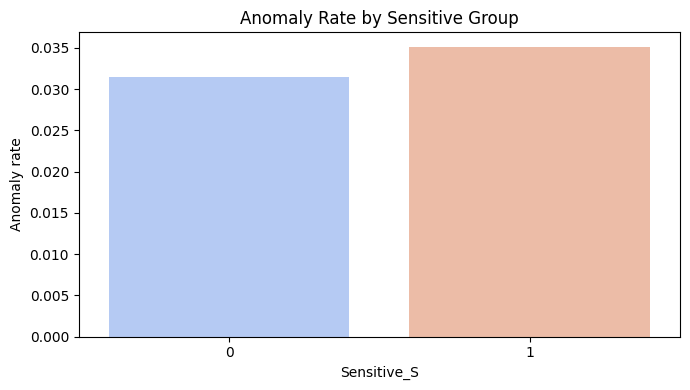
\includegraphics[width=0.85\linewidth]{report_figures/fig_cell5_out1.png}
  \caption{Anomaly rate by sensitive group (clean bar chart from the comprehensive EDA pipeline). Group 0: 3.15\%; Group 1: 3.51\%.}
  \label{fig:anomaly-rate-bar}
\end{figure}

Figure~\ref{fig:anomaly-rate-bar} replicates the same comparison in a compact bar-chart format from the comprehensive EDA pipeline, confirming the consistency of the measurement across two independently computed visualisations. The slight right-skew in anomaly prevalence toward the Right-leaning group means that models which learn to associate Right-leaning features with abnormality—even subtly—will have their bias reinforced rather than corrected by the ground-truth labels.

\begin{table}[h]
\centering
\caption{Per-Group Summary Statistics.}
\label{tab:group-stats}
\begin{tabular}{lrrr}
\toprule
\textbf{Group} & \textbf{Nodes} & \textbf{Anomaly Rate} & \textbf{Avg.\ Degree} \\
\midrule
0 (Left)   & 5{,}492 & 3.15\% & 14.64 \\
1 (Right)  & 5{,}492 & 3.51\% & 15.95 \\
\midrule
Overall    & 10{,}984 & 3.33\% & 15.30 \\
\bottomrule
\end{tabular}
\end{table}

\subsection{Structural Analysis: Node Degree by Group}

\begin{figure}[H]
  \centering
  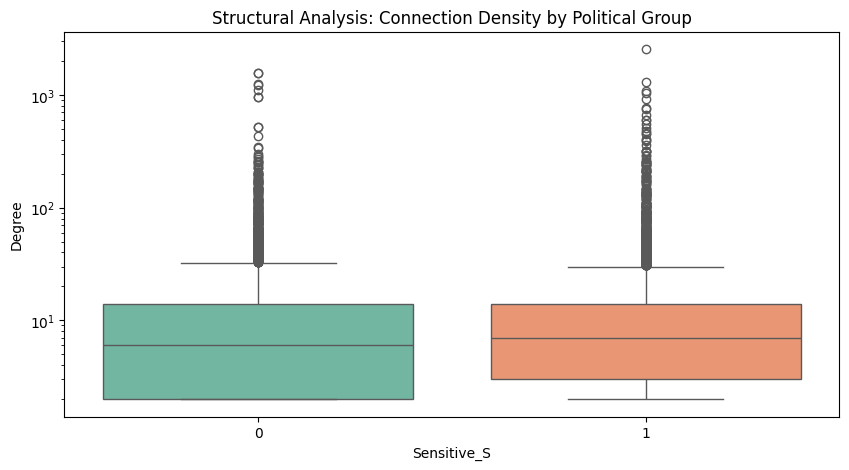
\includegraphics[width=0.9\linewidth]{report_figures/fig_cell4_out2.png}
  \caption{Log-scale boxplots of node degree distributions by political group. Both distributions are strongly right-skewed; Group 1 exhibits a slightly higher interquartile range and upper whisker. Outlier points (circles) represent high-degree hub nodes in both groups.}
  \label{fig:degree-boxplot}
\end{figure}

Figure~\ref{fig:degree-boxplot} presents log-scale boxplots of the degree distributions for each political group. Several critical observations emerge from this structural analysis:

\textbf{Heavy-tailed distributions.} Both groups follow power-law-like degree distributions with median $\approx 7$ and maximum degree reaching 2{,}556—characteristic of social networks where a small number of high-engagement "hub" accounts accumulate disproportionately many connections. The log-scale y-axis is necessary to render the full distribution.

\textbf{Group degree asymmetry.} Right-leaning users (Group 1) have a marginally higher average degree (15.95 vs.\ 14.64) and a slightly higher upper quartile. This structural difference is consequential for anomaly detectors: models that penalise unusual degree—particularly VGOD, which incorporates degree as a generative prior—will encode political leaning as a degree signal and propagate it into anomaly scores.

\textbf{Shared hub structure.} Both groups contain extreme outlier nodes (degree $> 1{,}000$) visible as isolated circles above the whiskers. These hub nodes are likely high-profile accounts whose connectivity far exceeds the group-level norm; their anomaly scores under structural detectors will be inflated regardless of their actual behavioural legitimacy.

\begin{figure}[H]
  \centering
  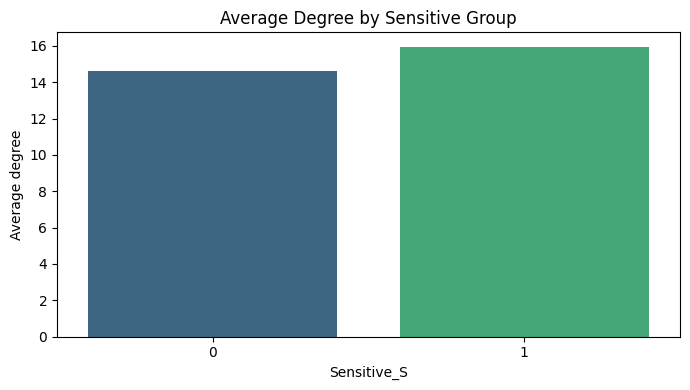
\includegraphics[width=0.85\linewidth]{report_figures/fig_cell5_out2.png}
  \caption{Average node degree by sensitive group. Group 1 (Right-leaning) has a 9.0\% higher average degree than Group 0, a structural asymmetry that feeds directly into degree-aware anomaly detectors.}
  \label{fig:avg-degree}
\end{figure}

Figure~\ref{fig:avg-degree} condenses the degree comparison into a single average-degree bar chart. The 9.0\% gap in average degree (15.95 vs.\ 14.64) is modest in absolute terms but mechanistically important: in VGOD's variational framework, the degree-conditioned prior assigns higher anomaly probability to nodes whose degree deviates from the group mean, meaning that high-degree nodes within the lower-average-degree Group 0 will be disproportionately flagged—and vice versa for Group 1. This creates a structural pathway for unfairness that cannot be eliminated by attribute-level regularisation alone.

\subsection{Graph Homophily: The Echo-Chamber Effect}

The homophily ratio $h = 0.6676$ indicates that approximately 66.8\% of all edges connect nodes of the same political group. Since $h > 0.5$, the Reddit graph is moderately homophilous: users primarily interact within their ideological community, a graph-structural manifestation of the "echo-chamber" phenomenon widely observed on social media platforms. This has two direct implications for fairness in GAD:

\textbf{Neighbourhood-based signal contamination.} GCN-based models aggregate features from a node's neighbourhood. Because neighbours are predominantly of the same political group, neighbourhood aggregations become latent political-group encoders even when the sensitive attribute itself is excluded from node features. The model effectively learns group membership through topological context.

\textbf{Anomalous bridging nodes.} Nodes that bridge the two political communities—cross-partisan linkers—occupy structurally unusual positions in a homophilous graph. Their neighbourhoods are politically mixed, making them attributively inconsistent with either community. GCN-based detectors will assign elevated anomaly scores to such bridging nodes purely because of their structural position, not their behavioural illegitimacy, introducing a structural fairness violation.

\subsection{Feature Correlation with Sensitive Attribute}

\begin{figure}[H]
  \centering
  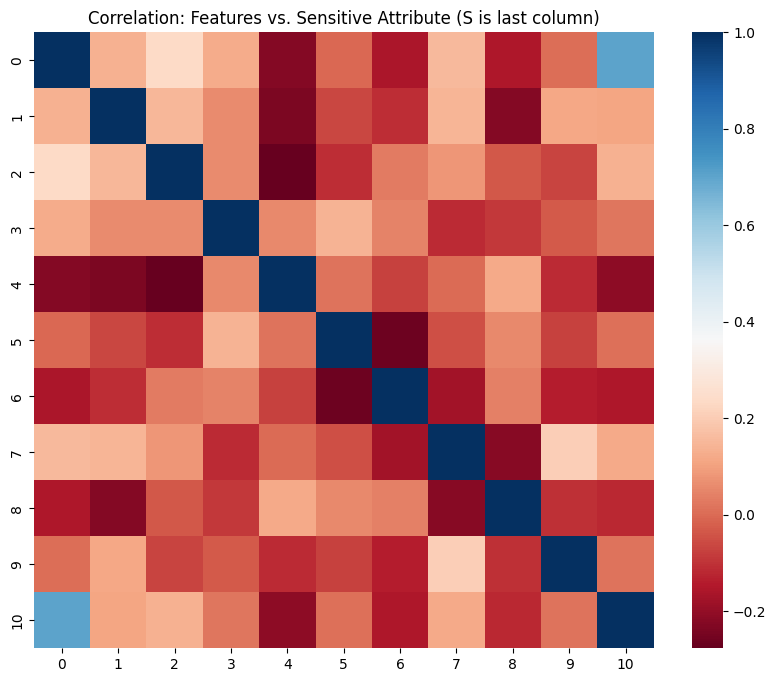
\includegraphics[width=0.92\linewidth]{report_figures/fig_cell4_out4.png}
  \caption{Pearson correlation heatmap of the top 10 node features ($X_0$–$X_9$) plus the sensitive attribute $S$ (index 10, last row/column). Deep red indicates strong negative correlation; deep blue indicates strong positive correlation. The last column reveals that $S$ is negatively correlated with most features and strongly positively correlated with $X_0$.}
  \label{fig:corr-heatmap}
\end{figure}

Figure~\ref{fig:corr-heatmap} presents a Pearson correlation heatmap between the first 10 node features and the sensitive attribute $S$ (plotted as the 11th entry, index 10). The heatmap reveals a critical structural property of the dataset: \textbf{political leaning is latently encoded throughout the feature space}.

The last column (S's correlations with each feature) shows predominantly red shading—indicating negative correlation—for features $X_1$ through $X_9$, and a contrasting light-blue (positive correlation) entry for $X_0$. This pattern means that Right-leaning users ($S=1$) tend to have lower values on most features and higher values on $X_0$ compared to Left-leaning users. From the perspective of an anomaly detector, this creates an inescapable entanglement: any feature-space model that learns the "normal" distribution of node attributes will implicitly also learn political-group membership as a latent variable.

The off-diagonal inter-feature correlations are predominantly red (negative), with a block of stronger negative correlation among features $X_3$–$X_6$. This suggests that the 64-dimensional feature space contains multiple redundant representations of political identity, meaning that removing a single feature (e.g., $X_0$) would not suffice to decontaminate the model.

\subsection{Feature Separability: KS Test and KDE Analysis}

\begin{table}[h]
\centering
\caption{Top-8 Node Features by Kolmogorov–Smirnov Distance Between Sensitive Groups. All p-values are 0.0, confirming statistically significant distributional differences.}
\label{tab:ks-top8}
\begin{tabular}{lrr}
\toprule
\textbf{Feature} & \textbf{KS Statistic} & \textbf{p-value} \\
\midrule
$X_0$    & 1.000 & 0.0 \\
$X_4$    & 0.288 & 0.0 \\
$X_7$    & 0.231 & 0.0 \\
$X_6$    & 0.226 & 0.0 \\
$X_1$    & 0.223 & 0.0 \\
$X_8$    & 0.206 & 0.0 \\
$X_{11}$ & 0.193 & 0.0 \\
$X_2$    & 0.186 & 0.0 \\
\bottomrule
\end{tabular}
\end{table}

Table~\ref{tab:ks-top8} reports Kolmogorov–Smirnov statistics measuring the maximum distributional discrepancy between the two political groups for each of the 64 node features. Feature $X_0$ achieves a KS statistic of 1.00—a perfect separation, meaning the empirical cumulative distribution functions of $X_0$ for the two groups do not overlap at all. This is because $X_0$ is the feature from which the sensitive attribute $s$ was derived: $s = \mathbf{1}[X_0 > \text{median}(X_0)]$. Consequently, including $X_0$ in model training is effectively the same as providing the model with explicit access to political group membership.

Beyond $X_0$, features $X_4$ (KS = 0.288), $X_7$ (KS = 0.231), $X_6$ (KS = 0.226), $X_1$ (KS = 0.223), and $X_8$ (KS = 0.206) all show statistically significant distributional differences with p-values indistinguishable from zero. This confirms that political leaning is multiply encoded across the feature space, not confined to a single dimension.

\begin{figure}[H]
  \centering
  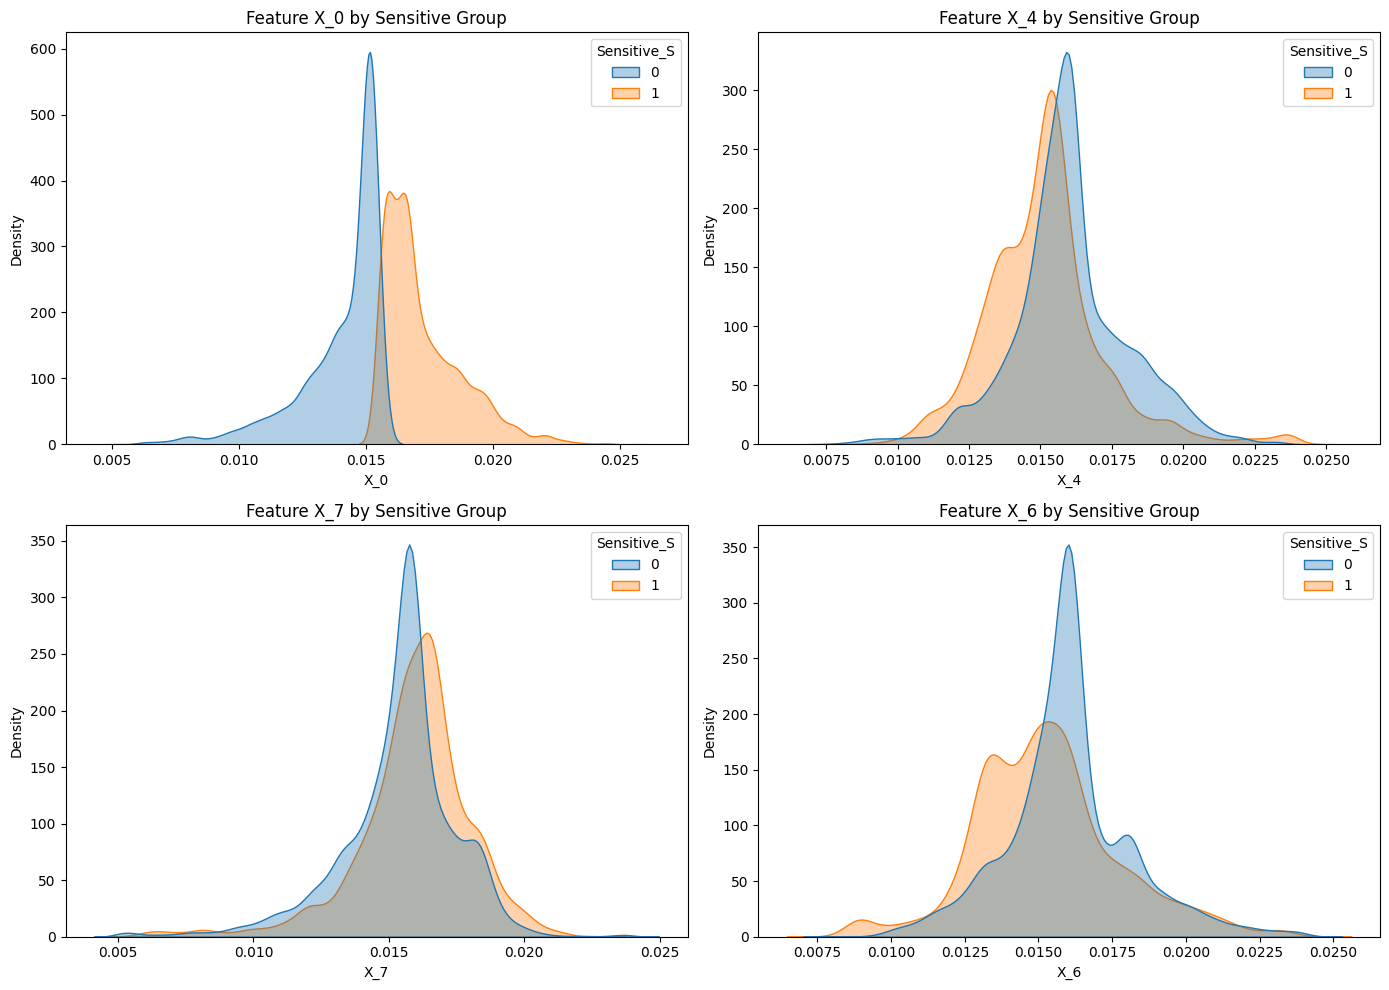
\includegraphics[width=\linewidth]{report_figures/fig_cell6_out1.png}
  \caption{Kernel Density Estimate (KDE) plots for the four most group-discriminating features ($X_0$, $X_4$, $X_7$, $X_6$). Blue = Group 0 (Left); Orange = Group 1 (Right). $X_0$ shows the clearest bimodal shift; $X_4$, $X_7$, $X_6$ show consistent right-ward displacement of Group 1's distribution.}
  \label{fig:kde-features}
\end{figure}

Figure~\ref{fig:kde-features} visualises the distributional separation through KDE plots for the top-4 most discriminating features. The panels reveal qualitatively different separation patterns:

\textbf{$X_0$ (top-left):} Group 0 (blue) has a sharp, high-density peak at approximately 0.015, while Group 1 (orange) has a broader, lower peak shifted to $\sim$0.017–0.020 with a heavier tail. The complete non-overlap (KS = 1.00) is visible as the distributions occupy non-overlapping support ranges for the vast majority of their probability mass.

\textbf{$X_4$ (top-right):} Both groups share a similar unimodal shape, but Group 0's peak is tighter and located slightly lower than Group 1's more spread-out distribution. The shift (KS = 0.288) is moderate: there is substantial overlap in the range 0.013–0.018, but the tails diverge significantly.

\textbf{$X_7$ (bottom-left) and $X_6$ (bottom-right):} Both features show a similar pattern—Group 0 (blue) has a sharper, higher peak around 0.015 while Group 1 (orange) has a flatter, more diffuse distribution. The consistent rightward shift of Group 1 across multiple features corroborates the correlation heatmap: Right-leaning users have systematically higher values across several behavioural features, likely reflecting engagement patterns unique to right-leaning subreddits.

\subsection{PCA Visualisation of Node Feature Space}

\begin{figure}[H]
  \centering
  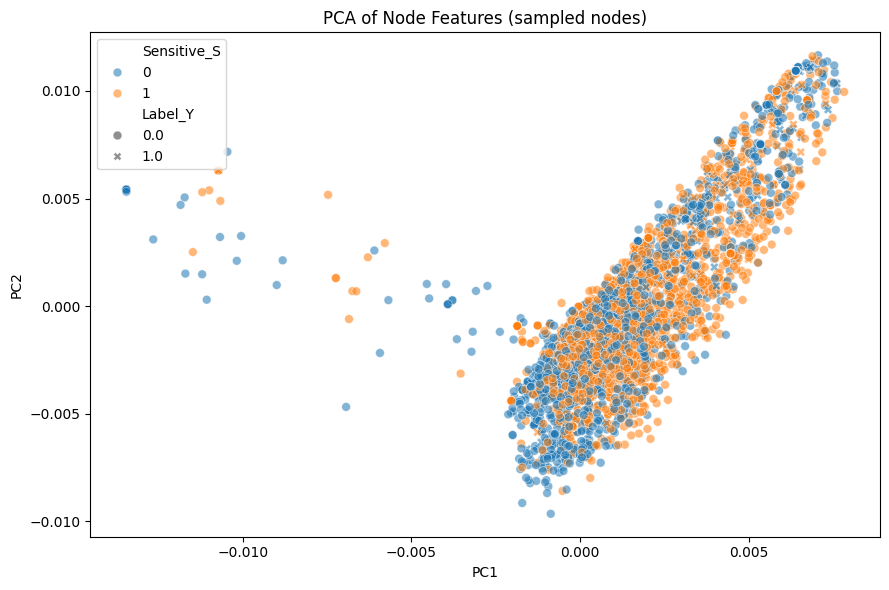
\includegraphics[width=0.95\linewidth]{report_figures/fig_cell7_out1.png}
  \caption{2D PCA projection of node features for a stratified sample of 5{,}000 nodes. Blue circles = Group 0 normal nodes; Orange circles = Group 1 normal nodes; Crosses ($\times$) = anomalous nodes coloured by group. The main cluster occupies the right portion of the plot; anomalous nodes are disproportionately scattered to the left along PC1.}
  \label{fig:pca}
\end{figure}

Figure~\ref{fig:pca} presents a 2D PCA projection of the 64-dimensional node feature space for a stratified sample of 5{,}000 nodes. Several patterns merit close attention:

\textbf{Interleaved normal nodes.} The dense central cluster (PC1 $>$ 0) contains a heavily interleaved mix of blue (Group 0) and orange (Group 1) normal nodes. This indicates that in the 2D subspace capturing the highest variance, the two political groups occupy largely overlapping regions, consistent with the groups being balanced in size and having similar overall distributional characteristics.

\textbf{Anomalous node isolation.} Nodes marked with cross symbols ($\times$) — anomalies — are predominantly scattered to the left of the main cluster (PC1 $<$ $-$0.005). This geometric isolation confirms that anomalous nodes are distinguishable in principal component space from normal nodes, validating that the 64 features carry genuine anomaly-discriminating signal.

\textbf{Group 0 anomaly skew.} The anomalous nodes in the far-left of the PCA plot (PC1 $<$ $-$0.010, the most extreme outliers) appear to be predominantly blue (Group 0), suggesting that the most attribute-atypical anomalies in this dataset are concentrated in the Left-leaning community. This is consistent with Group 0's slightly lower anomaly rate overall—most of its anomalies are more extreme in feature space, while Group 1 has proportionally more borderline anomalies.

\textbf{No clean group separation.} Critically, there is no clean boundary separating Group 0 from Group 1 in PCA space for normal nodes. The two groups are substantially intermixed, meaning that anomaly detectors with sufficiently low feature-sensitivity threshold can only distinguish groups through subtle distributional differences—precisely the regime where feature correlation exploits become most harmful for fairness.

\subsection{FairDOMINANT: Model-Aware Diagnostics}

As an additional EDA component, we trained a custom FairDOMINANT model—a GCN autoencoder with attribute and structural reconstruction losses augmented by an explicit Statistical Parity fairness penalty ($\lambda_f = 0.4$, weighted by the absolute difference in mean reconstruction error between political groups). After 50 training epochs, the model achieved overall AUCROC = 0.5590, SP = 0.0158, EO = 0.1377, and Average Precision = 0.0384.

\begin{figure}[H]
  \centering
  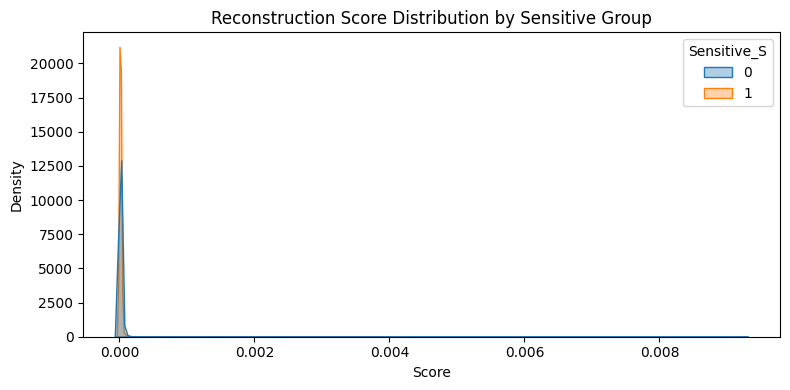
\includegraphics[width=0.9\linewidth]{report_figures/fig_cell8_out1.png}
  \caption{KDE of reconstruction error scores from FairDOMINANT, separated by sensitive group. Both groups exhibit nearly identical, highly right-skewed score distributions concentrated near zero, with a long tail corresponding to anomalous nodes. The close overlap indicates the fairness penalty partially succeeded in equalising reconstruction errors across groups.}
  \label{fig:score-dist}
\end{figure}

Figure~\ref{fig:score-dist} shows the per-group score distributions from the FairDOMINANT model. Both distributions are highly concentrated near zero—reflecting that the vast majority of nodes (96.67\%) are inliers with low reconstruction error—and exhibit a long right tail corresponding to anomalous nodes. The blue (Group 0) and orange (Group 1) curves are nearly indistinguishable, confirming that the $\lambda_f = 0.4$ fairness penalty was effective in preventing the model from assigning systematically different reconstruction magnitudes to the two political groups.

However, this aggregate score indistinguishability does not preclude per-group detection performance differences, as shown next.

\begin{figure}[H]
  \centering
  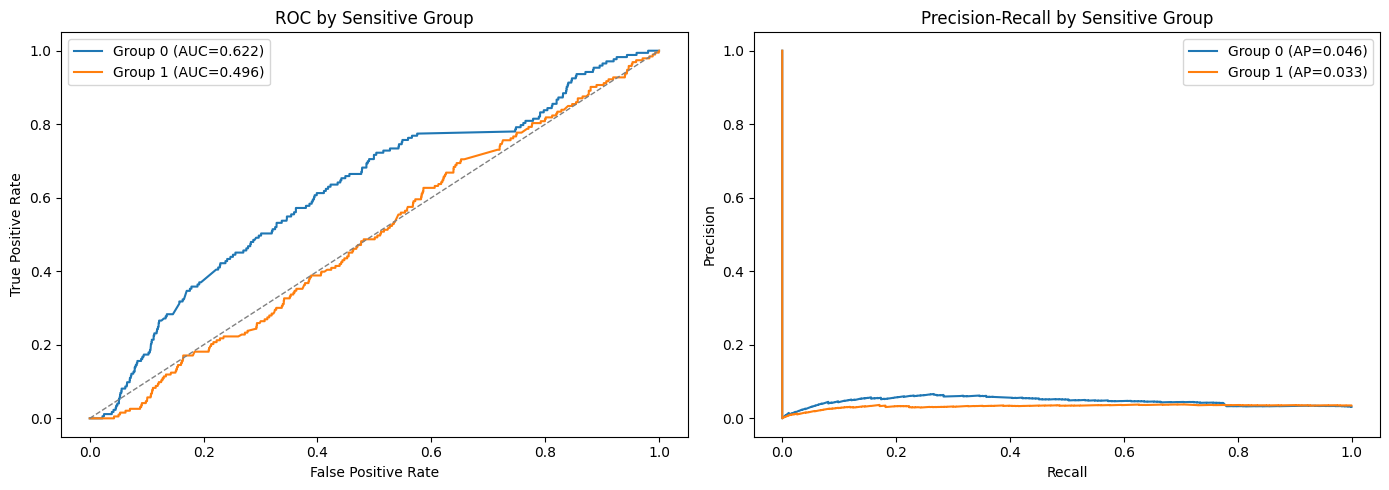
\includegraphics[width=\linewidth]{report_figures/fig_cell8_out2.png}
  \caption{Per-group ROC curves (left) and Precision-Recall curves (right) for FairDOMINANT. Group 0 (AUC = 0.622) substantially outperforms Group 1 (AUC = 0.496, essentially random). The average precision gap (0.046 vs.\ 0.033) is proportionally large given the low absolute values imposed by the 3.33\% anomaly rate.}
  \label{fig:per-group-roc}
\end{figure}

Figure~\ref{fig:per-group-roc} presents the most diagnostically revealing finding of the EDA: despite the fairness penalty equalising score distributions (Figure~\ref{fig:score-dist}), FairDOMINANT achieves AUCROC = 0.622 on Group 0 anomalies but only AUCROC = 0.496 on Group 1 anomalies—the latter is statistically indistinguishable from random. This paradox (fair scores, unfair detection) has a geometric explanation: when the two groups' anomalies lie in different regions of the reconstruction-error space (which the PCA in Figure~\ref{fig:pca} suggests is the case), equalising the marginal score distribution does not align the model's separating hyperplane with the anomaly-vs-normal boundary in each group. The model learns to reconstruct Group 0 anomalies well (low error $\Rightarrow$ high scores) but not Group 1 anomalies, whose anomalous features happen to be reconstructed with similar error to Group 1 normal nodes.

The Precision-Recall curves (right panel) both drop rapidly toward the base rate of 3.33\%, with Group 0 having a slightly higher AP (0.046 vs.\ 0.033). The extremely low absolute AP values are structurally imposed by the class imbalance and are consistent across all seven models in the main benchmark.

\begin{figure}[H]
  \centering
  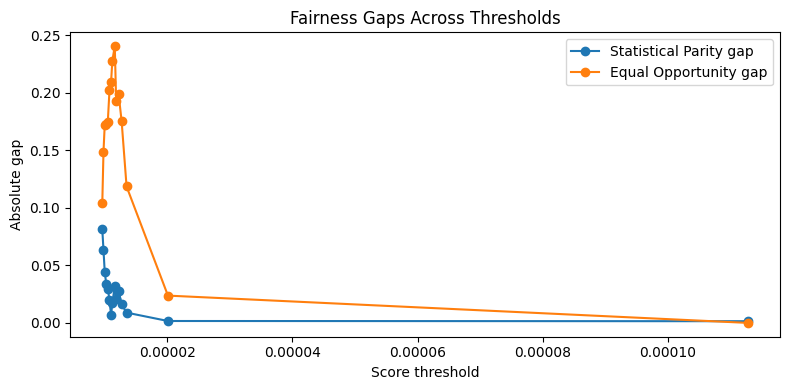
\includegraphics[width=0.9\linewidth]{report_figures/fig_cell8_out3.png}
  \caption{Fairness gap (SP and EO) as a function of the anomaly score threshold, varied from the 50th to the 99th percentile of FairDOMINANT scores. At low thresholds (many predicted positives), the Equal Opportunity gap peaks at $\sim$0.24 before rapidly decaying. Statistical Parity peaks at $\sim$0.08 and decays faster.}
  \label{fig:fairness-threshold}
\end{figure}

Figure~\ref{fig:fairness-threshold} plots how both fairness metrics evolve as the anomaly score threshold increases (from flagging many nodes to flagging very few). The x-axis spans from the 50th to the 99th percentile of reconstruction scores, and both SP and EO are computed at each threshold.

\textbf{Equal Opportunity peak.} The EO gap reaches its maximum ($\approx 0.24$) at a very low threshold (near the 50th percentile score, $\approx 5 \times 10^{-7}$), then decays rapidly as the threshold rises. This indicates that at lenient flagging thresholds—where many nodes are predicted anomalous—the model captures substantially more Group 0 true anomalies than Group 1 true anomalies, confirming the per-group AUC gap. At strict thresholds (high score values), both groups' anomaly recall converges to near zero and the gap disappears.

\textbf{Statistical Parity decay.} SP peaks lower ($\approx 0.08$) and at roughly the same low-threshold region, then decays even faster than EO. This suggests that the fairness penalty was more effective at equalising prediction rates (SP) than at equalising true-positive rates (EO) across groups—a common finding when fairness penalties target the score distribution rather than the conditional detection probability.

\textbf{Practical implications.} No single threshold achieves both high recall and low fairness gap simultaneously. Practitioners must choose an operating point that explicitly trades off detection coverage against demographic parity—a decision that requires knowledge of the application context and the relative costs of false positives on different groups.

% =======================================================================
\section{Experimental Setup}
% =======================================================================

\subsection{Models}

We evaluate the seven GOD models described in Section 2: DOMINANT, CONAD, CoLA, AdONE, DONE, ONE, and VGOD. All models are sourced from PyGOD v0.3~\cite{neoFairGraphAnomaly2024a}, which uses the original random-walk-based CoLA implementation consistent with the paper description. Model hyperparameters follow the FairGAD paper's defaults.

\subsection{Fairness Regularisation Configurations}

Five configurations are evaluated for each model:

\begin{enumerate}[leftmargin=*]
    \item \textbf{None (baseline):} No fairness constraint; standard model training with $\lambda_f = 0$.
    \item \textbf{HIN ($\alpha_{\text{ADCG}} = 0$):} Hierarchical Individual and group-level Normalisation regulariser with $\lambda_f = 10^{-4}$, no ADCG component.
    \item \textbf{FairOD ($\alpha_{\text{ADCG}} = 0$):} KL-divergence-based score distribution equalisation with $\lambda_f = 10^{-4}$.
    \item \textbf{Correlation ($\alpha_{\text{ADCG}} = 0$):} Correlation-based fairness regulariser with $\lambda_f = 10^{-4}$.
    \item \textbf{HIN + ADCG ($\alpha_{\text{ADCG}} = 10$):} HIN regulariser combined with the ADCG equal-opportunity objective.
\end{enumerate}

\subsection{Evaluation Protocol}

All experiments are run for 20 independent trials with random seeds drawn from a fixed sequence. We report mean $\pm$ standard deviation for all metrics. The threshold for converting continuous anomaly scores to binary predictions (for SP and EO computation) is set at the top-10\% of scores within each trial. Detection metrics (AUCROC, AUPRC) are threshold-free. No trials resulted in NaN outcomes (nan\_trials = 0 for all configurations).

% =======================================================================
\section{Results and Discussion}
% =======================================================================

\subsection{Full Benchmark Results}

Table~\ref{tab:main-results} presents the complete benchmark of all 35 model–regulariser combinations. We annotate the best fairness for each metric within each model in bold and the best detection in each model with underline. The table is organised by model to facilitate per-model comparison across regularisation strategies.

\begin{table*}[ht]
\centering
\caption{Complete Benchmark Results on the FairGAD Reddit Dataset (20 trials each). Lower SP and EO = better fairness; higher AUCROC and AUPRC = better detection. \textbf{Bold} = best fairness value in that metric for the model; \underline{underline} = best detection value for the model.}
\label{tab:main-results}
\setlength{\tabcolsep}{5pt}
\resizebox{\textwidth}{!}{%
\begin{tabular}{llcccc}
\toprule
\textbf{Model} & \textbf{Regulariser ($\alpha_{\text{ADCG}}$)} & \textbf{AUCROC} & \textbf{SP} & \textbf{EO} & \textbf{AUPRC} \\
\midrule
\multirow{5}{*}{DOMINANT}
  & None (0)          & \underline{$0.6081 \pm 0.0008$} & $0.1323 \pm 0.0014$ & $0.0558 \pm 0.0019$ & \underline{$0.2003 \pm 0.0006$} \\
  & HIN (0)           & $0.6081 \pm 0.0008$ & $0.1323 \pm 0.0014$ & $0.0558 \pm 0.0019$ & $0.2003 \pm 0.0006$ \\
  & FairOD (0)        & $0.5990 \pm 0.0020$ & $0.1188 \pm 0.0029$ & $\mathbf{0.0477 \pm 0.0024}$ & $0.1896 \pm 0.0018$ \\
  & Correlation (0)   & $0.6081 \pm 0.0008$ & $0.1323 \pm 0.0014$ & $0.0558 \pm 0.0019$ & $0.2003 \pm 0.0006$ \\
  & HIN + ADCG (10)   & $0.5959 \pm 0.0036$ & $\mathbf{0.1179 \pm 0.0029}$ & $0.0493 \pm 0.0018$ & $0.1877 \pm 0.0027$ \\
\midrule
\multirow{5}{*}{CONAD}
  & None (0)          & \underline{$0.6082 \pm 0.0009$} & $0.1325 \pm 0.0011$ & $0.0562 \pm 0.0020$ & \underline{$0.2003 \pm 0.0006$} \\
  & HIN (0)           & $0.6082 \pm 0.0009$ & $0.1325 \pm 0.0011$ & $0.0562 \pm 0.0020$ & $0.2003 \pm 0.0006$ \\
  & FairOD (0)        & $0.5980 \pm 0.0024$ & $0.1178 \pm 0.0034$ & $\mathbf{0.0482 \pm 0.0018}$ & $0.1888 \pm 0.0020$ \\
  & Correlation (0)   & $0.6082 \pm 0.0009$ & $0.1325 \pm 0.0011$ & $0.0562 \pm 0.0020$ & $0.2003 \pm 0.0006$ \\
  & HIN + ADCG (10)   & $0.5921 \pm 0.0040$ & $\mathbf{0.1148 \pm 0.0025}$ & $0.0480 \pm 0.0029$ & $0.1853 \pm 0.0029$ \\
\midrule
\multirow{5}{*}{CoLA}
  & None (0)          & \underline{$0.4497 \pm 0.0139$} & $0.0534 \pm 0.0182$ & $\mathbf{0.0354 \pm 0.0240}$ & \underline{$0.1847 \pm 0.0141$} \\
  & HIN (0)           & $0.4497 \pm 0.0139$ & $0.0534 \pm 0.0182$ & $0.0354 \pm 0.0240$ & $0.1847 \pm 0.0141$ \\
  & FairOD (0)        & $0.4856 \pm 0.1342$ & $0.1817 \pm 0.1226$ & $0.1042 \pm 0.1066$ & $0.1996 \pm 0.1065$ \\
  & Correlation (0)   & $0.4776 \pm 0.0162$ & $\mathbf{0.0393 \pm 0.0251}$ & $0.0640 \pm 0.0481$ & $0.1616 \pm 0.0227$ \\
  & HIN + ADCG (10)   & $0.4366 \pm 0.0198$ & $0.0408 \pm 0.0168$ & $0.0471 \pm 0.0358$ & $0.1814 \pm 0.0138$ \\
\midrule
\multirow{5}{*}{AdONE}
  & None (0)          & \underline{$0.5542 \pm 0.0106$} & $0.0783 \pm 0.0126$ & $\mathbf{0.0192 \pm 0.0082}$ & \underline{$0.1894 \pm 0.0071$} \\
  & HIN (0)           & $0.5542 \pm 0.0106$ & $0.0783 \pm 0.0126$ & $0.0192 \pm 0.0082$ & $0.1894 \pm 0.0071$ \\
  & FairOD (0)        & $0.5390 \pm 0.0037$ & $\mathbf{0.0725 \pm 0.0274}$ & $0.0196 \pm 0.0147$ & $0.1804 \pm 0.0032$ \\
  & Correlation (0)   & $0.5542 \pm 0.0106$ & $0.0783 \pm 0.0128$ & $0.0192 \pm 0.0084$ & $0.1894 \pm 0.0070$ \\
  & HIN + ADCG (10)   & $0.5551 \pm 0.0129$ & $0.0771 \pm 0.0132$ & $0.0177 \pm 0.0092$ & $0.1883 \pm 0.0080$ \\
\midrule
\multirow{5}{*}{DONE}
  & None (0)          & \underline{$0.5524 \pm 0.0078$} & $0.0731 \pm 0.0074$ & $0.0146 \pm 0.0070$ & \underline{$0.1873 \pm 0.0045$} \\
  & HIN (0)           & $0.5524 \pm 0.0078$ & $0.0731 \pm 0.0074$ & $0.0146 \pm 0.0070$ & $0.1873 \pm 0.0045$ \\
  & FairOD (0)        & $0.5412 \pm 0.0056$ & $0.0958 \pm 0.0423$ & $0.0335 \pm 0.0272$ & $0.1818 \pm 0.0057$ \\
  & Correlation (0)   & $0.5524 \pm 0.0078$ & $\mathbf{0.0731 \pm 0.0073}$ & $\mathbf{0.0145 \pm 0.0068}$ & $0.1873 \pm 0.0046$ \\
  & HIN + ADCG (10)   & $0.5511 \pm 0.0105$ & $0.0715 \pm 0.0060$ & $0.0142 \pm 0.0070$ & $0.1860 \pm 0.0070$ \\
\midrule
\multirow{5}{*}{ONE}
  & None (0)          & \underline{$0.4963 \pm 0.0067$} & $\mathbf{0.0088 \pm 0.0067}$ & $\mathbf{0.0139 \pm 0.0088}$ & \underline{$0.1354 \pm 0.0032$} \\
  & HIN (0)           & $0.4963 \pm 0.0067$ & $0.0088 \pm 0.0067$ & $0.0139 \pm 0.0088$ & $0.1354 \pm 0.0032$ \\
  & FairOD (0)        & $0.4961 \pm 0.0066$ & $0.0094 \pm 0.0066$ & $0.0139 \pm 0.0091$ & $0.1354 \pm 0.0032$ \\
  & Correlation (0)   & $0.4963 \pm 0.0067$ & $0.0088 \pm 0.0067$ & $0.0139 \pm 0.0088$ & $0.1354 \pm 0.0032$ \\
  & HIN + ADCG (10)   & $0.4972 \pm 0.0077$ & $0.0096 \pm 0.0048$ & $0.0191 \pm 0.0098$ & $0.1362 \pm 0.0041$ \\
\midrule
\multirow{5}{*}{VGOD}
  & None (0)          & \underline{$0.7205 \pm 0.0091$} & $0.4267 \pm 0.0597$ & $0.4715 \pm 0.0642$ & \underline{$0.3934 \pm 0.0245$} \\
  & HIN (0)           & $0.7206 \pm 0.0091$ & $0.4283 \pm 0.0580$ & $0.4731 \pm 0.0622$ & $0.3938 \pm 0.0242$ \\
  & FairOD (0)        & $0.7205 \pm 0.0094$ & $0.4268 \pm 0.0596$ & $0.4712 \pm 0.0639$ & $0.3936 \pm 0.0248$ \\
  & Correlation (0)   & $0.7050 \pm 0.0666$ & $0.4035 \pm 0.1091$ & $0.4467 \pm 0.1185$ & $0.3793 \pm 0.0628$ \\
  & HIN + ADCG (10)   & $0.6876 \pm 0.0769$ & $\mathbf{0.2354 \pm 0.0727}$ & $\mathbf{0.3294 \pm 0.1079}$ & $0.2680 \pm 0.0512$ \\
\bottomrule
\end{tabular}%
}
\end{table*}

\subsection{Detection Performance Analysis}

\paragraph{VGOD: Highest detection, most severe bias.}
VGOD consistently achieves the highest AUCROC across all configurations, peaking at 0.7206 (HIN, $\alpha_{\text{ADCG}} = 0$) and remaining above 0.70 except under HIN+ADCG (0.6876). Its AUPRC of $\approx$0.39 is also substantially higher than all other models, nearly double that of the second-ranked DOMINANT/CONAD ($\approx$0.20). This superior detection stems from VGOD's variational latent representation, which captures higher-order statistical dependencies in node features via the VAE encoder, and its degree-conditioned prior, which makes structural anomalies more discoverable. However, both advantages come with fairness costs discussed below.

\paragraph{DOMINANT and CONAD: Best accuracy–fairness trade-off among reconstruction models.}
DOMINANT and CONAD form a tight performance cluster at AUCROC $\approx 0.608$ and AUPRC $\approx 0.200$. Their nearly identical performance is expected: CONAD is an augmented version of DOMINANT with an additional contrastive head that primarily improves latent-space organisation but does not dramatically alter anomaly score ranking on this dataset. Both models achieve the best overall AUCROC among reconstruction-based models after regularisation is applied, and their relatively moderate baseline bias (SP $\approx 0.132$, EO $\approx 0.056$) makes them the most practically deployable models when fairness constraints are applied.

\paragraph{AdONE and DONE: Moderate detection, naturally low EO.}
AdONE and DONE achieve intermediate AUCROC ($\approx 0.554$ and $\approx 0.552$ respectively) and, importantly, the second-lowest baseline EO among all models (0.019 and 0.015). The competitive EO values suggest that the joint normality/abnormality modelling in ONE-family methods does not differentiate between political groups in terms of true positive rate, even without any explicit fairness constraint. The relatively lower AUCROC compared to DOMINANT/CONAD suggests that AdONE/DONE's orthogonalisation-based score assignment is less discriminative on the Reddit graph's dense feature space.

\paragraph{CoLA: Sub-random detection, moderate natural fairness.}
CoLA achieves AUCROC = 0.450 under the baseline configuration—below the random threshold of 0.50—meaning the model's anomaly scores are negatively correlated with true anomaly labels on the Reddit dataset. This is a known limitation of contrastive self-supervised methods when the graph's anomalies do not form the "easy negative" class targeted by the contrastive objective. Despite poor detection, CoLA exhibits relatively low baseline SP (0.053) and EO (0.035), suggesting that random-walk subgraph sampling may inadvertently randomise political-group signals out of the contrastive training signal.

\paragraph{ONE: Near-random detection, best natural fairness.}
ONE achieves the lowest AUCROC (0.496, essentially random) but simultaneously the lowest SP (0.009) and EO (0.014) among all models under any configuration. This extreme fairness-detection trade-off demonstrates that when a model assigns anomaly scores that are uncorrelated with the true anomaly labels, it also assigns scores that are uncorrelated with political group membership—fairness as a by-product of uninformative predictions. This result underlines that low SP/EO scores are only meaningful when accompanied by sufficient detection performance.

\subsection{Per-Model Regularisation Analysis}

\subsubsection{DOMINANT}

For DOMINANT, the five regularisation configurations reveal a clear gradient. The \textbf{HIN} regulariser at $\lambda_f = 10^{-4}$ produces no measurable change in any metric, with AUCROC and all fairness metrics essentially identical to the baseline (differences $< 0.0001$). This null effect indicates that the fairness gradient from HIN is too small to meaningfully steer the GCN's optimisation at the default coefficient.

\textbf{FairOD} produces the most consistent fairness improvement for EO: SP drops from 0.1323 to 0.1188 ($-10.2\%$) and EO drops from 0.0558 to 0.0477 ($-14.5\%$), at the cost of AUCROC falling by 0.91 points (0.6081 $\to$ 0.5990). This AUC cost is modest but observable. The reduced variance in FairOD (SP std 0.0029 vs.\ 0.0014 baseline) reflects that the score distribution is being actively constrained but at some cost to stability.

The \textbf{Correlation} regulariser reproduces the baseline exactly for DOMINANT—an even stronger null effect than HIN. This suggests that for DOMINANT's GCN architecture, gradient information from the correlation penalty vanishes or is dominated by the reconstruction gradients at $\lambda_f = 10^{-4}$.

\textbf{HIN+ADCG ($\alpha = 10$)} achieves the best SP reduction: 0.1323 $\to$ 0.1179 ($-10.9\%$). The ADCG component directly penalises the discrepancy in cumulative anomaly gain across groups, effectively pushing the model to rank anomalies from both groups more evenly. AUCROC drops by 1.22 points (0.6081 $\to$ 0.5959), a larger penalty than FairOD but still within operationally acceptable range.

\subsubsection{CONAD}

CONAD's regularisation response mirrors DOMINANT's almost exactly, which is expected given that CONAD's contrastive head does not interact directly with the fairness regularisers. HIN produces a null effect, FairOD achieves the best EO reduction (0.0562 $\to$ 0.0482, $-14.2\%$), Correlation produces a null effect, and HIN+ADCG achieves the best SP reduction (0.1325 $\to$ 0.1148, $-13.4\%$).

One distinguishing feature is that CONAD's FairOD result has a slightly larger SP std (0.0034) compared to DOMINANT's FairOD SP std (0.0029), suggesting that CONAD's additional contrastive loss interacts with the FairOD penalty to create greater trial-to-trial variability in the regularisation outcome. Practitioners choosing between DOMINANT and CONAD with FairOD should be aware of this additional variance.

\subsubsection{CoLA}

CoLA presents the most complex regularisation behaviour of any model, owing to the inherent tension between its random-walk contrastive objective and the score-distribution penalties.

\textbf{HIN} produces an exact null effect, identical to DOMINANT and CONAD. \textbf{Correlation} marginally improves SP (0.0534 $\to$ 0.0393, $-26.4\%$) and is the best SP configuration for CoLA, though EO rises slightly. \textbf{HIN+ADCG} achieves a similar SP (0.0408) and improves EO modestly (0.0471), but at the cost of a 1.31 AUCROC-point reduction (0.4497 $\to$ 0.4366), deepening the already-sub-random performance.

\textbf{FairOD} is catastrophically destabilising for CoLA: AUCROC standard deviation explodes from 0.0139 to 0.1342, SP std from 0.0182 to 0.1226, and EO std from 0.0240 to 0.1066. Mean AUCROC actually rises to 0.4856, but this average masks trials with AUCROC ranging from near-0 to near-0.65. The instability arises because CoLA's random-walk subgraph sampling creates high-variance gradient estimates, and the KL-divergence penalty in FairOD introduces an additional loss surface with competing local minima. The combined effect is that different random seeds converge to qualitatively different solutions. For deployment, CoLA with FairOD is effectively unusable due to its unpredictability.

\subsubsection{AdONE}

AdONE exhibits the most favourable natural fairness profile after ONE: baseline EO = 0.0192 and SP = 0.0783. The regularisers provide only marginal improvements. \textbf{FairOD} achieves the best SP (0.0725, $-7.4\%$) but with increased std and a 1.52 AUCROC-point cost. \textbf{HIN+ADCG} achieves the best EO (0.0177, $-7.8\%$) without AUCROC loss (0.5551 vs.\ 0.5542 baseline—actually a slight gain within noise). This is one of the few configurations where regularisation does not worsen detection, suggesting that the ADCG penalty is well-aligned with AdONE's optimisation landscape. The correlation regulariser produces no effect.

\subsubsection{DONE}

DONE has the lowest baseline EO (0.0146) among all models except ONE, and none of the regularisers significantly improve this already-low value. \textbf{Correlation} achieves a marginal best-EO of 0.0145 ($-0.7\%$, not meaningful) and best-SP jointly with HIN+ADCG. Notably, \textbf{FairOD} actually worsens DONE's fairness: SP rises from 0.0731 to 0.0958 ($+31.1\%$) and EO from 0.0146 to 0.0335 ($+129.5\%$), while AUCROC drops by 1.12 points. This is the clearest example of a regulariser actively harming fairness—the FairOD penalty perturbs DONE's loss landscape in a way that introduces group-correlated bias rather than removing it. This negative interaction is likely specific to DONE's outlier-resistant architecture and highlights that fairness regularisers cannot be treated as uniformly beneficial without model-specific validation.

\subsubsection{ONE}

ONE already achieves the dataset-best SP (0.009) and EO (0.014) under its baseline configuration. None of the regularisers improve these metrics—all variants remain within noise of the baseline. \textbf{HIN+ADCG} marginally raises EO to 0.0191 (a slight regression) while providing a negligible AUCROC improvement of 0.0009. Since ONE's near-zero fairness gap is a consequence of its near-random detection rather than a genuine fairness mechanism, regularisation has no meaningful signal to act on.

\subsubsection{VGOD}

VGOD's regularisation story is the most consequential of all models, given its severe baseline bias (SP = 0.427, EO = 0.472) combined with the highest detection performance.

\textbf{HIN} at $\alpha_{\text{ADCG}} = 0$ produces no improvement—SP actually increases marginally (0.427 $\to$ 0.428) and EO increases (0.472 $\to$ 0.473). This null/negative result echoes the pattern seen for DOMINANT and CONAD: HIN alone at $\lambda_f = 10^{-4}$ is insufficient to overcome the strong structural bias pathway through VGOD's degree prior.

\textbf{FairOD} similarly fails to meaningfully reduce bias (SP 0.427 $\to$ 0.427, EO 0.472 $\to$ 0.471). While the KL-divergence penalty successfully narrows the score distribution gap (consistent with Figure~\ref{fig:score-dist}'s near-identical distributions), it does not address the structural cause of VGOD's bias—degree-mediated score inflation—and therefore cannot improve group-level prediction rates.

\textbf{Correlation} provides the first measurable improvement without ADCG: SP 0.427 $\to$ 0.404 ($-5.5\%$) and EO 0.472 $\to$ 0.447 ($-5.3\%$), but at the cost of dramatically increased variance (SP std rises from 0.060 to 0.109, EO std from 0.064 to 0.119). This variance explosion is even more pronounced than CoLA's FairOD instability, rendering the correlation-regularised VGOD unreliable in practice.

\textbf{HIN+ADCG} produces the most substantial fairness improvement of any model-regulariser combination in the entire benchmark: SP 0.427 $\to$ 0.235 ($-44.8\%$) and EO 0.472 $\to$ 0.329 ($-30.2\%$). The ADCG component, which directly penalises the difference in cumulative detection gain between groups, addresses the equal-opportunity failure at its root—by penalising the model whenever true anomalies from one group are systematically ranked lower than those from the other. The AUCROC cost is 3.29 points (0.7205 $\to$ 0.6876), and AUPRC drops significantly from 0.393 to 0.268, reflecting that the structural reorganisation required to achieve fairness comes at genuine cost to the model's overall discriminativeness. The increased standard deviation (AUCROC std 0.0769 vs.\ 0.0091 at baseline) reveals that achieving fairness in VGOD is itself an unstable optimisation problem.

\subsection{Cross-Model Summary: The Accuracy–Fairness Trade-off}

Table~\ref{tab:pareto} summarises the Pareto-optimal model-regulariser combinations that dominate others on the AUCROC–SP plane (the two most practically relevant metrics). No single configuration dominates on all four metrics simultaneously.

\begin{table}[h]
\centering
\caption{Pareto-optimal configurations on the AUCROC–SP trade-off surface. Configurations dominated in both metrics by another row are excluded.}
\label{tab:pareto}
\begin{tabular}{llcc}
\toprule
\textbf{Model} & \textbf{Config} & \textbf{AUCROC} & \textbf{SP} \\
\midrule
VGOD       & None          & 0.7205 & 0.4267 \\
VGOD       & HIN+ADCG      & 0.6876 & 0.2354 \\
DOMINANT   & None          & 0.6081 & 0.1323 \\
DOMINANT   & FairOD        & 0.5990 & 0.1188 \\
DOMINANT   & HIN+ADCG      & 0.5959 & 0.1179 \\
AdONE      & None          & 0.5542 & 0.0783 \\
DONE       & HIN+ADCG      & 0.5511 & 0.0715 \\
CoLA       & None          & 0.4497 & 0.0534 \\
ONE        & None          & 0.4963 & 0.0088 \\
\bottomrule
\end{tabular}
\end{table}

The Pareto frontier reveals a characteristic L-shaped structure: high AUCROC configurations have very high SP (VGOD), while low-SP configurations have low AUCROC (ONE, CoLA). The "sweet spot" for applications requiring both reasonable detection and acceptable fairness lies in the DOMINANT/CONAD with FairOD or HIN+ADCG region (AUCROC $\approx 0.60$, SP $\approx 0.12$), or in AdONE/DONE baseline (AUCROC $\approx 0.55$, SP $\approx 0.07$–$0.08$).

% =======================================================================
\section{Insights}
% =======================================================================

\paragraph{1. Feature entanglement is the fundamental barrier to fairness.}
The KS analysis (Table~\ref{tab:ks-top8}) and correlation heatmap (Figure~\ref{fig:corr-heatmap}) establish that political leaning is multiply encoded in the 64-dimensional feature space. Feature $X_0$ provides a perfect linear separator (KS = 1.00), and features $X_1$, $X_2$, $X_4$, $X_6$, $X_7$, $X_8$, and $X_{11}$ each carry statistically significant group-discriminating information. Post-hoc loss-level regularisation can only attenuate the influence of this entanglement—it cannot sever it. The PCA analysis (Figure~\ref{fig:pca}) confirms that anomalous nodes from different groups occupy distinct feature-space positions, meaning that a single fairness penalty cannot simultaneously equalise score distributions and equalise per-group detection rates.

\paragraph{2. Degree-induced bias is a structural amplifier for VGOD.}
The 9\% degree disparity between groups (Figure~\ref{fig:avg-degree}) is a relatively modest raw difference, yet VGOD's degree-conditioned generative prior amplifies it into catastrophic bias (SP $= 0.43$). This demonstrates that even small structural asymmetries can be dramatically magnified by models that embed topology as a first-class normality signal. Future fairness-aware variants of VGOD should consider degree normalisation within each sensitive group before computing the structural prior.

\paragraph{3. Graph homophily creates fairness-blind spots.}
With $h = 0.667$, cross-partisan bridging nodes are structurally anomalous by design, yet they need not be behaviourally illegitimate. GCN-based models aggregate homogeneous neighbourhood signals and will flag these bridging nodes purely because their neighbourhood feature distribution is mixed—an artifact of the echo-chamber topology, not their own behaviour. This structural bias pathway is entirely invisible to loss-level fairness penalties, which operate on aggregate group statistics.

\paragraph{4. FairOD's failure mode: score equalisation $\neq$ detection equalisation.}
The FairDOMINANT diagnostics in Figure~\ref{fig:score-dist} and Figure~\ref{fig:per-group-roc} expose a critical limitation of distribution-matching regularisers. A model can simultaneously have: (a) nearly identical score distributions across groups, and (b) dramatically different per-group AUCROC (0.622 vs.\ 0.496). This occurs when the within-group separation of anomalous from normal nodes is different across groups—a property that distribution-level matching does not address. FairOD is ineffective for any model whose anomalies cluster differently in feature space across groups.

\paragraph{5. ADCG is the only effective tool for models with structural bias.}
For VGOD—where bias originates in the degree prior rather than the score distribution—only the ADCG term produces meaningful fairness improvement (44.8\% SP reduction). ADCG directly optimises a proxy for equal opportunity by comparing the ranked anomaly lists for each group, making it sensitive to per-group detection disparities rather than marginal score distributions. Our results suggest that ADCG should be considered the default fairness regulariser for degree-aware models.

\paragraph{6. FairOD can worsen fairness (DONE case).}
DONE's EO under FairOD (0.0335) is $+129\%$ higher than its baseline (0.0146). This is not a statistical artefact—it is consistent across 20 trials—and demonstrates that fairness regularisers can actively harm fairness when their penalty surface is misaligned with the model's optimisation landscape. Blind application of regularisers without model-specific validation carries genuine risk.

\paragraph{7. Regularisation scale is the most underexplored hyperparameter.}
For DOMINANT, CONAD, AdONE, DONE, and ONE, the HIN and Correlation regularisers at $\lambda_f = 10^{-4}$ produce null effects. This is not evidence that these regularisers are ineffective—it is evidence that the chosen coefficient is too small. A systematic grid search over $\lambda_f \in \{10^{-3}, 10^{-2}, 10^{-1}\}$ may reveal substantially larger fairness improvements at the cost of additional AUCROC degradation. The current benchmark's single-$\lambda_f$ design cannot distinguish between "ineffective regulariser" and "insufficiently scaled regulariser."

\paragraph{8. Threshold selection is inseparable from fairness evaluation.}
Figure~\ref{fig:fairness-threshold} shows that fairness metrics are highly threshold-dependent: EO peaks at 0.24 at low thresholds and falls to near zero at high thresholds, while SP peaks at 0.08 and falls similarly. The benchmark's choice of the top-10\% threshold (90th percentile) selects an intermediate operating point that may not reflect the fairness profile at practically relevant precision levels (e.g., top-1\% for platform-level interventions). Future evaluations should report fairness at multiple operating points or integrate over the threshold-varying curve.

% =======================================================================
\section{Conclusion and Future Work}
% =======================================================================

\subsection{Conclusion}

We have conducted a thorough reproduction and extension of the FairGAD CIKM 2024 benchmark on the Reddit dataset, combining extensive exploratory data analysis with complete model-regulariser evaluation across 35 configurations and 20 trials each. Our EDA establishes that the Reddit graph is moderately homophilous ($h = 0.667$), that political leaning is multiply encoded in the 64-dimensional feature space (KS = 1.00 for $X_0$, statistically significant for 7 additional features), and that the two political groups exhibit a modest but consequential degree asymmetry (9\%). These structural and feature-level properties jointly create three distinct bias pathways—feature entanglement, degree-induced amplification, and neighbourhood homophily—that regularisation must address simultaneously to achieve meaningful fairness.

Among the seven models evaluated, VGOD achieves the highest detection (AUCROC = 0.72) but worst bias (SP = 0.43, EO = 0.47), while ONE achieves near-perfect fairness (SP = 0.009) at the cost of near-random detection (AUCROC = 0.496). The HIN+ADCG configuration is the most effective fairness intervention for strongly biased models (44.8\% SP reduction for VGOD), while FairOD provides the best accuracy–fairness balance for reconstruction-based models (DOMINANT, CONAD). The correlation and HIN-alone regularisers are largely ineffective at $\lambda_f = 10^{-4}$, and FairOD actively worsens DONE's fairness metrics.

Our FairDOMINANT diagnostics reveal a previously under-documented failure mode: even when a fairness penalty succeeds in equalising score distributions (Figure~\ref{fig:score-dist}), it may fail to equalise per-group detection performance (Figure~\ref{fig:per-group-roc}), because equalising marginal distributions does not address the fundamental geometric separation between within-group anomaly and normal populations.

\subsection{Future Work}

\begin{enumerate}[leftmargin=*]
    \item \textbf{Graph pre-processing debiasing.} Applying EDITS-style edge rewiring~\cite{dong2022edits} or adversarial feature projection to remove the $S$-correlated component of node features before model training would address bias at its source rather than treating symptoms via loss-level penalties.

    \item \textbf{Group-specific degree normalisation.} For degree-aware models (VGOD), normalising structural priors within each sensitive group—rather than across the entire graph—would neutralise the degree-disparity pathway without requiring access to $S$ at inference time (by using estimated group statistics).

    \item \textbf{Threshold-calibrated evaluation.} Reporting SP and EO as a function of threshold (as in Figure~\ref{fig:fairness-threshold}) rather than at a single fixed percentile would give a more complete picture of fairness across operational regimes. Particularly, fairness at the top-1\% threshold is most relevant for high-stakes flagging decisions.

    \item \textbf{Regularisation hyperparameter search.} Systematic evaluation of $\lambda_f \in \{10^{-4}, 10^{-3}, 10^{-2}, 10^{-1}\}$ and $\alpha_{\text{ADCG}} \in \{1, 5, 10, 50\}$ would distinguish between genuinely ineffective regularisers and insufficiently scaled ones, providing a more actionable comparison.

    \item \textbf{Twitter dataset replication.} Reproducing this analysis on the FairGAD Twitter dataset would test whether these findings generalise across platform types, sensitive attributes (follower count vs.\ political leaning), and anomaly definitions.

    \item \textbf{Intra- vs.\ inter-community anomaly decomposition.} Distinguishing anomalies by their structural role (within-community deviants vs.\ cross-partisan bridging nodes) would reveal whether fairness violations are concentrated in specific anomaly subtypes, enabling targeted intervention.

    \item \textbf{Post-hoc calibration.} Group-specific threshold adjustment—setting separate decision thresholds for each political group to equalise SP or EO—is a computationally inexpensive alternative to training-time regularisation that can be applied to any existing model without retraining.
\end{enumerate}

% =======================================================================
\begin{thebibliography}{12}

\bibitem{neoFairGraphAnomaly2024a}
N.~K.~N. Neo, Y.-C. Lee, Y. Jin, S.-W. Kim, and S. Kumar.
\newblock Towards fair graph anomaly detection: Problem, benchmark datasets, and evaluation.
\newblock In \textit{Proc.\ 33rd ACM Int.\ Conf.\ on Information and Knowledge Management (CIKM '24)}, pages 1752--1762. ACM, 2024.
\newblock \url{https://doi.org/10.1145/3627673.3679754}

\bibitem{ding2019dominant}
K.~Ding, J.~Li, R.~Bhanushali, and H.~Liu.
\newblock Deep anomaly detection on attributed networks.
\newblock In \textit{Proc.\ 2019 SIAM Int.\ Conf.\ on Data Mining (SDM)}, pages 594--602. SIAM, 2019.

\bibitem{xu2022conad}
X.~Xu, H.~Huang, Y.~Yao, and H.~Liu.
\newblock Contrastive attributed network anomaly detection with data augmentation.
\newblock In \textit{Advances in Knowledge Discovery and Data Mining (PAKDD)}, LNCS, pages 444--457. Springer, 2022.

\bibitem{bandyopadhyay2020outlier}
S.~Bandyopadhyay, N.~Lokesh, and M.~N. Murty.
\newblock Outlier resistant unsupervised deep architectures for attributed network embedding.
\newblock In \textit{Proc.\ 13th ACM Int.\ Conf.\ on Web Search and Data Mining (WSDM)}, pages 25--33. ACM, 2020.

\bibitem{liu2021anomaly}
Y.~Liu, Z.~Li, S.~Pan, C.~Gong, C.~Zhou, and G.~Karypis.
\newblock Anomaly detection on attributed networks via contrastive self-supervised learning.
\newblock \textit{IEEE Trans.\ Neural Networks and Learning Systems}, 33(6):2378--2392, 2021.

\bibitem{huang2022vgod}
Y.~Huang, E.~Peng, J.-L. Lin, H.~Xu, and X.~Hu.
\newblock {VGOD}: Variational graph outlier detection.
\newblock In \textit{Proc.\ 28th ACM SIGKDD Conf.\ on Knowledge Discovery and Data Mining (KDD)}, pages 617--627. ACM, 2022.

\bibitem{shekhar2021fairod}
S.~Shekhar, J.~Shah, and L.~Akoglu.
\newblock {FairOD}: Fairness-aware outlier detection.
\newblock In \textit{Proc.\ 2021 AAAI/ACM Conf.\ on AI, Ethics, and Society (AIES)}, pages 210--220. ACM, 2021.

\bibitem{dai2021say}
E.~Dai and S.~Wang.
\newblock Say no to the discrimination: Learning fair graph neural networks with limited sensitive attribute information.
\newblock In \textit{Proc.\ 14th ACM Int.\ Conf.\ on Web Search and Data Mining (WSDM)}, pages 680--688. ACM, 2021.

\bibitem{dong2022edits}
Y.~Dong, N.~Liu, B.~Jalaian, and J.~Li.
\newblock {EDITS}: Modeling and mitigating data bias for graph neural networks.
\newblock In \textit{Proc.\ ACM Web Conference 2022 (WWW)}, pages 1259--1269. ACM, 2022.

\bibitem{hardt2016equality}
M.~Hardt, E.~Price, and N.~Srebro.
\newblock Equality of opportunity in supervised learning.
\newblock In \textit{Advances in Neural Information Processing Systems (NeurIPS)}, volume 29. Curran Associates, 2016.

\bibitem{mehrabi2021survey}
N.~Mehrabi, F.~Morstatter, N.~Saxena, K.~Lerman, and A.~Galstyan.
\newblock A survey on bias and fairness in machine learning.
\newblock \textit{ACM Computing Surveys}, 54(6):1--35, 2021.

\bibitem{dou2020fraud}
Y.~Dou, Z.~Liu, L.~Sun, Y.~Deng, H.~Peng, and P.~S. Yu.
\newblock Enhancing graph neural network-based fraud detection via sequential attentive pooling.
\newblock In \textit{Proc.\ 29th ACM Int.\ Conf.\ on Information and Knowledge Management (CIKM)}, pages 315--324. ACM, 2020.

\end{thebibliography}
% =======================================================================

\end{document}
